\documentclass[a4paper,12pt]{article}

\usepackage{graphicx}

\usepackage{graphicx}
\usepackage{geometry} % Modificar márgenes
\geometry{ % Especificación modificación márgenes
    a4paper,
    left=2cm,
    right=2cm,
    top=2cm,
    bottom=2cm
}
\usepackage[utf8]{inputenc}
\usepackage[spanish]{babel} % Paquete para escritura en español
\usepackage{float} % Etiqueta 'H' (mayus) en figuras (imágenes)
\usepackage{array} % Padding en tablas
\usepackage{url} % Etiqueta url en .bib
\usepackage{booktabs} % Manejo de caudros (tablas)
\usepackage[T1]{fontenc}    % Codificación de fuentes
\usepackage{csquotes}       % Paquete para comillas tipográficas

\begin{document}

\section{Objetivo}
Que el alumno conozca los principales aspectos teóricos y prácticos de las colecciones y sus aplicaciones en el lenguaje de programación Java, así mismo que ponga en práctica los conceptos básicos de la programación orientada a objetos.

\section{Introducción}

Una parte fundamental de cualquier programa son las colecciones de datos, es importante como programador conocer y estar familiarizado con cada manera que existe de almacenar información. Todo el análisis previo que se hace al iniciar un nuevo proyecto es de suma importancia y presenta el lugar y momento para definir ciertos aspectos fundamentales del programa, cuál es su función, qué va a realizar, cómo se va a organizar, qué se busca y cómo se va a implementar. Junto a estos aspectos y en este momento se definen qué colecciones se van a utilizar.

¿Qué colección necesito usar? Es una pregunta totalmente válida y muy necesaria de hacerse en el momento de crear un nuevo programa. Para tomar la decisión se debe tener muy en claro lo que se necesita, ¿qué operaciones se van a utilizar?, ¿se necesita iterar el almacenamiento únicamente?, ¿utilizas operación de búsqueda?, ¿cuán eficiente debe ser su rendimiento?, entre otros aspectos más específicos.

Es entonces indudable la importancia de dominar las colecciones al momento de crear un nuevo programa y ellas, a su vez, están estrechamente ligadas al lenguaje de programación elegido para desarrollar. Las colecciones en Java son herramientas fundamentales en el desarrollo de software, especialmente en el ámbito de la ingeniería de software. Estas colecciones son conjuntos de objetos que permiten el almacenamiento, manipulación y gestión eficiente de datos en programas Java.

En el presente trabajo se exploran las principales colecciones (interfaces e implementaciones) que existen en el lenguaje de programación con el que se trabaja en el curso: Java. En las páginas siguientes se encuentra una investigación sobre las colecciones más recurrentes en Java, un análisis detallado sobre el programa realizado (sistema de inscripción) para mostrar un uso práctico de dichas colecciones y afianzar los conocimientos en el tema, finalmente las conclusiones de cada integrante del equipo basado en lo obtenido.

\section{¿Qué son las colecciones en Java?}

Las colecciones en Java son conjuntos de objetos que permiten el almacenamiento, manipulación y gestión eficiente de datos en programas escritos en Java. Estas colecciones forman parte del Java Collections Framework (JCF) como se puede ver en la Figura 1, una biblioteca estándar incluida en el lenguaje de programación Java. El JCF ofrece una amplia gama de interfaces y clases predefinidas que permiten trabajar con diferentes tipos de estructuras de datos, como listas, conjuntos y mapas.

En esencia, las colecciones en Java nos proporcionan herramientas para almacenar y organizar grupos de elementos relacionados de manera eficiente. Por ejemplo, podemos utilizar una lista para almacenar una secuencia ordenada de elementos, un conjunto para almacenar elementos únicos sin duplicados, o un mapa para almacenar pares clave-valor.

La inclusión de las colecciones en el JCF facilita el desarrollo de aplicaciones Java al proporcionar implementaciones eficientes y optimizadas de estructuras de datos comunes. Esto permite a los programadores centrarse en la lógica de la aplicación en lugar de tener que implementar manualmente las estructuras de datos subyacentes.

Además, el JCF ofrece operaciones y algoritmos comunes para trabajar con colecciones, como agregar elementos, eliminar elementos, buscar elementos, ordenar colecciones y realizar otras operaciones de manipulación de datos. Esto simplifica el proceso de desarrollo y mejora la coherencia y la eficiencia del código.

\section{Principales colecciones en Java}

La jerarquía de colecciones en Java se establece de manera que cada nivel proporciona un conjunto específico de funcionalidades y comportamientos para manejar grupos de elementos de manera eficiente.

\subsection{Collection}

En la cima de esta jerarquía se encuentra la interfaz Collection, que sirve como la base para todas las colecciones en Java. Esta interfaz define operaciones comunes que se aplican a cualquier colección, como agregar, eliminar y comprobar la presencia de elementos.

Una colección representa un grupo de objetos, conocidos como elementos. Algunas colecciones permiten elementos duplicados y otras no. Algunas están ordenadas y otras desordenadas. El JDK no proporciona ninguna implementación directa de esta interfaz, sino que proporciona implementaciones de subinterfaces más específicas. Esta interfaz se utiliza normalmente para pasar colecciones y manipularlas cuando se desea la máxima generalidad. \cite{collection}

\subsection{Set}

Los Sets en Java constituyen una colección que no permite elementos duplicados, lo que significa que cada elemento es único en el conjunto. Estos conjuntos utilizan los métodos equals y hashCode para determinar la duplicidad de los elementos. Una implementación común de Sets es HashSet, que almacena los elementos en una tabla hash para permitir un acceso rápido y eficiente a los elementos.

Se debe tener cuidado de utilizar objetos mutables como elementos establecidos, pues el comportamiento de un conjunto no se especifica si el valor de un objeto se cambia de una manera en la que afecta comparaciones entre iguales mientras el objeto es un elemento del conjunto. Un caso especial de esta prohibición es que no está permitido que un conjunto se contenga a sí mismo como elemento.\cite{set}

\subsection{Map}

Por otro lado, los Maps en Java son estructuras que asocian claves con valores, creando pares clave-valor únicos. Esto implica que no puede haber claves duplicadas en un Map. HashMap es una implementación común de Map que utiliza una tabla hash internamente para almacenar los pares clave-valor, lo que proporciona un acceso rápido a los datos. Por otro lado, TreeMap es otra implementación de Map que utiliza una estructura de árbol de búsqueda para mantener las claves ordenadas.

Proporciona tres vistas de colección, permitiendo ver el contenido de un mapa como un conjunto de claves, una colección de valores, o un conjunto de asignaciones de valores-clave.\cite{map}

\subsection{List}

Además, las Lists en Java representan colecciones ordenadas de elementos donde se permite la duplicación de elementos y se mantiene el orden de inserción. ArrayList es una implementación común de List que almacena elementos en un arreglo dinámico, lo que permite un acceso rápido a los elementos mediante índices. Por otro lado, LinkedList es otra implementación de List que utiliza una lista doblemente enlazada, ofreciendo un rendimiento eficiente para la inserción y eliminación de elementos en cualquier posición. Estas colecciones en Java proporcionan una base sólida para el desarrollo de aplicaciones eficientes y escalables.

\subsection{Queue}

Otra subinterfaz importante es Queue, que representa una colección en la que los elementos se insertan en un extremo y se eliminan del otro extremo siguiendo el principio de FIFO (\textit{First-In, First-Out}). Esto la hace adecuada para implementaciones de colas, como \textit{PriorityQueue}.

Una colección diseñada para manejar elementos antes de su procesamiento. Además de las operaciones básicas de recopilación, las colas proporcionan operaciones adicionales de inserción, extracción e inspección. \cite{queue}

\begin{figure}[ht]
    \centering
    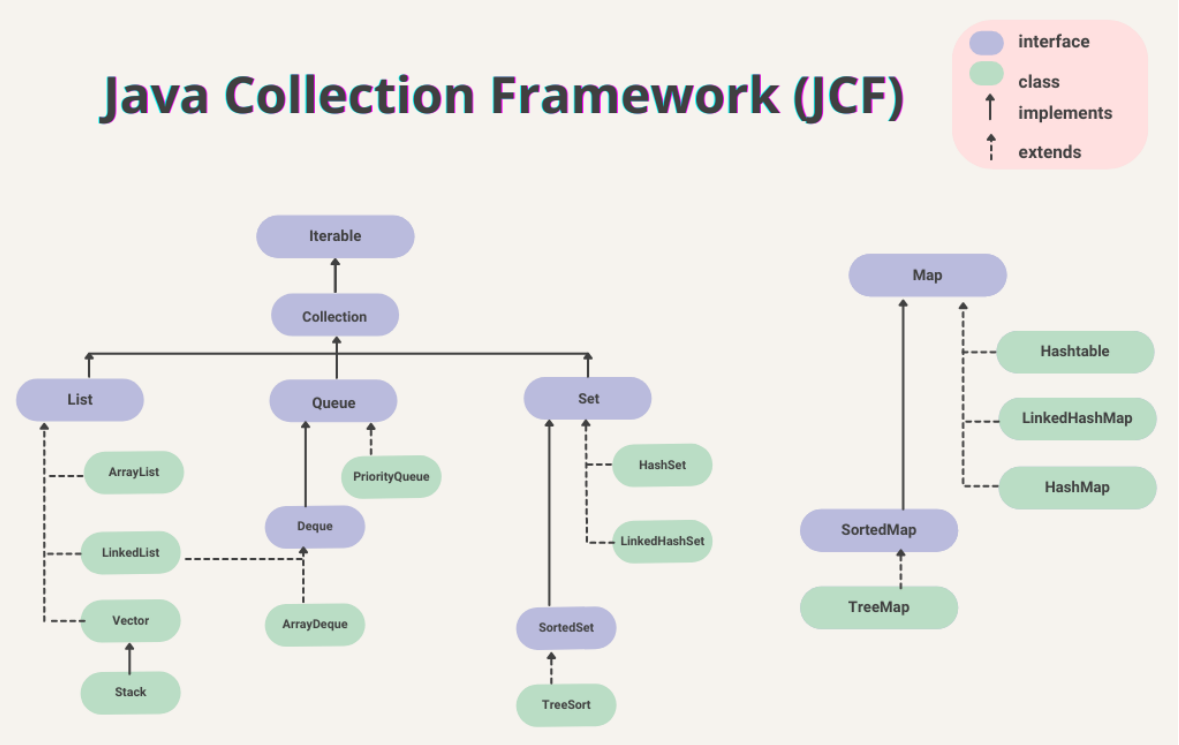
\includegraphics[width=.9\textwidth]{media/java_collection_framework.PNG}
    \caption{Java Collection Framework. \cite{nieva-2023}}
    \label{fig:enter-label}
\end{figure}

\section{Principales implementaciones (Clases)}

Las clases que implementan las interfaces de colecciones en Java ofrecen funcionalidades específicas para diferentes tipos de almacenamiento y manipulación de datos.

Además de las interfaces, también hay clases concretas que implementan estas interfaces y proporcionan funcionalidades específicas. Por ejemplo, ArrayList y LinkedList son implementaciones de la interfaz List, mientras que HashSet y TreeSet son implementaciones de la interfaz Set. HashMap y TreeMap son implementaciones de la interfaz Map, que representa una colección de pares clave-valor.

\subsection{ArrayList}

El ArrayList es una de las implementaciones más utilizadas de la interfaz List, que almacena los elementos en un arreglo dinámico. Esto permite un acceso rápido a los elementos mediante índices, aunque las operaciones de inserción y eliminación pueden ser costosas en términos de rendimiento, especialmente para grandes conjuntos de datos.

Implementa todas las operaciones de lista opcionales y permite todos los elementos, incluido el nulo. Además de implementar la interfaz List, esta clase proporciona métodos para manipular el tamaño de la matriz que se utiliza internamente para almacenar la lista. \cite{array_list}

Cada instancia de ArrayList tiene una capacidad. La capacidad es el tamaño de la matriz utilizada para almacenar los elementos de la lista. Siempre es al menos tan grande como el tamaño de la lista. A medida que se agregan elementos, su capacidad crece automáticamente.  \cite{array_list}

Es importante mencionar que esta implementación no está sincronizada, lo que significa que, si varios subprocesos acceden a una instancia de ArrayList simultáneamente y al menos uno de ellos realiza cualquier operación que agregue o elimine uno o más elementos, o cambia explícitamente el tamaño de la matriz (modificaciones estructurales), se debe sincronizar externamente. \cite{array_list}

\subsection{LinkedList}

Por otro lado, LinkedList es otra implementación de la interfaz List que utiliza una lista doblemente enlazada. Si bien ofrece un rendimiento eficiente para la inserción y eliminación de elementos en cualquier posición, acceder a elementos por índice puede ser menos eficiente que en ArrayList.

Todas las operaciones se realizan como se podría esperar de una lista doblemente enlazada. Las operaciones que indexan la lista recorrerán la lista desde el principio o el final, lo que esté más cerca del índice especificado.\cite{linked_list} De manera exactamente igual a como sucede con ArrayList, la implementación no está sincronizada y se debe sincronizar externamente de realizar modificaciones estructurales un subproceso.

\subsection{HashSet}

HashSet es una implementación de la interfaz Set que almacena elementos en una tabla hash (en realidad es una instancia de HashMap), lo que garantiza un acceso rápido a los elementos y la prohibición de elementos duplicados. Esta implementación es ideal cuando se necesita una colección sin elementos duplicados y el orden de los elementos no es importante, pues no garantiza que el orden se mantendrá constante en el tiempo, ni en cuanto al orden de iteración del conjunto.

Permite el elemento nulo y ofrece un rendimiento constante para las operaciones básicas (agregar, eliminar, contener y dimensionar), suponiendo que la función hash disperse los elementos adecuadamente entre los depósitos (\textit{bucket}). De manera exactamente igual a como sucede con LinkedList y ArrayList, la implementación no está sincronizada y se debe sincronizar externamente de realizar modificaciones estructurales un subproceso. \cite{hash_set}

\subsection{TreeSet}

TreeSet, por otro lado, es otra implementación de la interfaz Set que almacena elementos en un árbol de búsqueda ordenado. Esto garantiza que los elementos se mantengan ordenados según un criterio especificado, lo que puede ser útil en ciertas situaciones donde se necesita mantener un orden específico en la colección.

Los elementos se ordenan utilizando su orden natural o mediante un Comparador proporcionado en el momento de la cración establecido, según el constructor que se utilice. Esta implementación proporciona un costo de tiempo $log(n)$ garantizado para las operaciones básicas (agregar, eliminar y verificar existencia). \cite{tree_set}

\subsection{HashMap}

Para las implementaciones de la interfaz Map, HashMap es una implementación común que utiliza una tabla hash para almacenar pares clave-valor, lo que permite un acceso rápido a los valores a través de las claves a cambio de no ofrecer garantías en cuanto al orden del mapa.

Una instancia de HashMap tiene dos parámetros que afectan su rendimiento: capacidad inicial y factor de carga. La capacidad es la cantidad de depósitos en la tabla hash y la capacidad inicial es simplemente la capacidad en el momento en que se crea la tabla hash. El factor de carga es una medida de qué tan llena se permite que esté la tabla hash antes de que su capacidad aumente automáticamente. Cuando el número de entradas en la tabla hash excede el producto del factor de carga y la capacidad actual, la tabla hash se repite (es decir, se reconstruyen las estructuras de datos internas) para que la tabla hash tenga aproximadamente el doble de la cantidad de depósitos. \cite{hash_map}

\subsection{TreeMap}

Por otro lado, TreeMap es otra implementación de la interfaz Map que utiliza un árbol de búsqueda para mantener las claves ordenadas, lo que puede ser útil en situaciones donde se necesita mantener un orden específico en las claves.

El mapa se ordena según el orden natural de sus claves o mediante un comparador proporcionado en el momento de la creación del mapa, según el constructor que se utilice.
Esta implementación proporciona un costo de tiempo de $log(n)$ garantizado para las operaciones contiene clave, obtener, colocar y eliminar. \cite{tree_map}

Hay que tener en cuenta que esta implementación no está sincronizada. Si varios subprocesos acceden a un mapa al mismo tiempo y al menos uno de los subprocesos modifica el mapa estructuralmente, debe sincronizarse externamente. \cite{tree_map}

\section{Principales diferencias entre las implementaciones}

Es importante comprender las diferencias fundamentales entre las implementaciones de colecciones en Java, ya que estas diferencias afectan el rendimiento y la eficiencia de nuestros programas.

En primer lugar, en el caso de ArrayList y LinkedList, la diferencia radica en cómo se almacenan los elementos. ArrayList utiliza un arreglo dinámico, lo que permite un acceso rápido a los elementos mediante índices, pero las inserciones y eliminaciones pueden ser costosas. Por otro lado, LinkedList utiliza una lista doblemente enlazada, lo que facilita las inserciones y eliminaciones en cualquier posición, pero puede ser menos eficiente para el acceso aleatorio.

En cuanto a HashSet y TreeSet, la distinción principal está en cómo se organizan los elementos y se garantiza la unicidad. HashSet utiliza una tabla hash, ofreciendo un acceso rápido a los elementos y prohibiendo duplicados, pero no garantiza ningún orden particular de los elementos. Por otro lado, TreeSet utiliza un árbol de búsqueda, lo que garantiza que los elementos se mantengan ordenados y únicos, aunque puede ser un poco más lento debido a las operaciones de ordenación internas.

Por último, en el caso de HashMap y TreeMap, la diferencia principal radica en la organización de las claves. HashMap utiliza una tabla hash para un acceso rápido a los valores a través de las claves, sin garantizar un orden particular de las claves. Por otro lado, TreeMap utiliza un árbol de búsqueda para mantener las claves ordenadas, garantizando un orden específico de las claves, pero potencialmente con un rendimiento ligeramente inferior debido a las operaciones de ordenación.


\section{Aspectos cruciales para la implementación de colecciones en Java en la resolución eficiente de problemas}

\subsection{Análisis de requisitos}

Antes de empezar a resolver un problema es importante entender qué tipo de datos necesitamos manejar. ¿Necesitamos una lista que mantenga un orden específico? ¿O tal vez un conjunto donde no se permitan elementos duplicados? Hay diferentes tipos de colecciones en Java para diferentes necesidades. Por ejemplo, si queremos buscar elementos de manera rápida podríamos elegir HashSet.

\begin{figure}[ht]
    \centering
    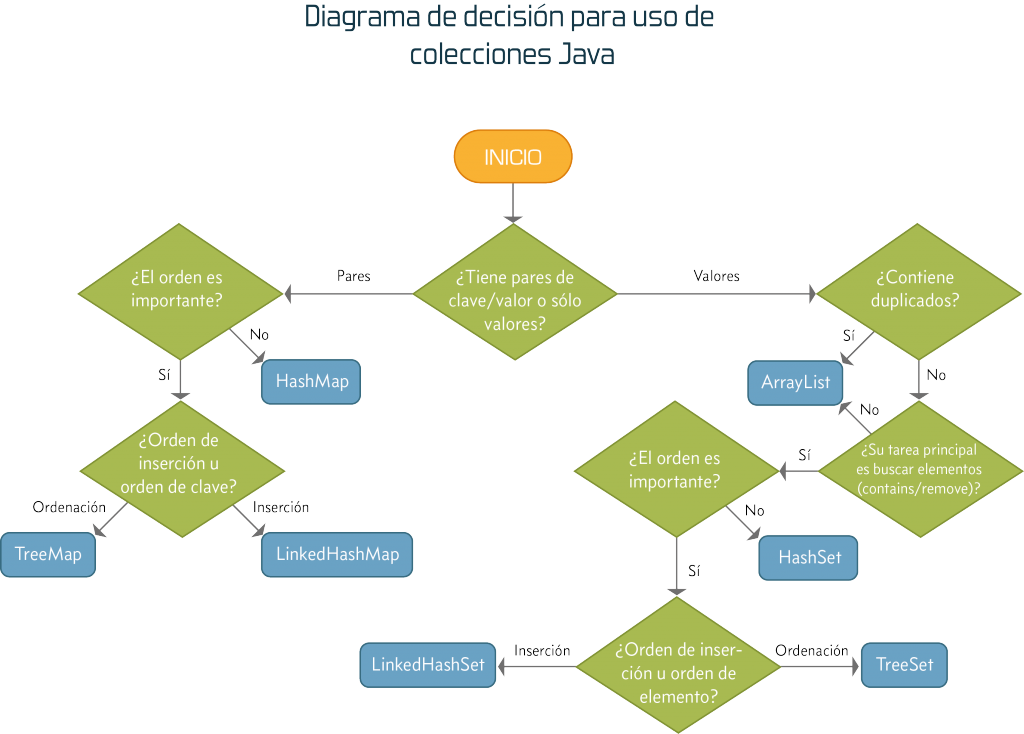
\includegraphics[width=.9\textwidth]{media/diagrama_decision_uso_de_colecciones.png}
    \caption{Diagrama de decisión para el uso de colecciones en Java. \cite{amor-2020}}
    \label{fig:diagrama_decision_colecciones}
\end{figure}

\subsection{Eficiencia temporal y espacial}

Cuando elijamos una colección, debemos pensar en cómo funcionará en términos de velocidad y espacio. ¿Qué tan rápido será para agregar, buscar o eliminar elementos? ¿Cuánta memoria utilizará? Por ejemplo, si usamos ArrayList, podemos acceder a los elementos rápidamente, pero si necesitamos agregar o eliminar elementos con frecuencia, LinkedList podría ser mejor.

\subsection{Manejo de duplicados}

A veces, no queremos que haya elementos repetidos en nuestra colección. En ese caso, podemos usar un conjunto (Set). Si necesitamos que los elementos se mantengan en un orden específico, podríamos usar LinkedHashSet.

\subsection{Iteración y recorrido}

Cuando necesitamos recorrer una colección, es importante hacerlo de manera eficiente. Podemos usar bucles especiales como el for-each. Pero debemos recordar que algunas colecciones, como HashSet, no garantizan un orden específico.

\subsection{Claves y valores en mapas}

Si necesitamos asociar claves con valores, podemos usar un mapa (Map). Es importante elegir claves únicas y significativas. Por ejemplo, si estamos usando HashMap, debemos asegurarnos de que nuestras claves sean únicas.

\subsection{Manejo de excepciones}

Al escribir código, siempre debemos estar preparados para manejar errores. Es importante considerar posibles excepciones como \textit{NullPointerException} o \textit{ConcurrentModificationException} y usar bloques \textit{try-catch} para manejarlas.

\subsection{Documentación y comentarios}

Finalmente, al escribir código es útil documentar lo que estamos haciendo y por qué lo estamos haciendo de esa manera. Esto ayuda a otros a entender nuestro código y también a nosotros mismos en el futuro. Es importante agregar comentarios para explicar nuestras decisiones de diseño.

\section{Análisis del programa}

El programa parte de idea de poder acceder mediante distintas interfaces\footnote{Como lo haría un usuario desde la comodidad de su hogar.} para un usuario de alumno o docente, adicionalmente y para tener acceso a todas las opciones se puede acceder como administrador. En los primeros dos casos es necesario tener una cuenta ingresada en el sistema para poder acceder a las funciones correspondientes, en el caso de ser administrador se da por entendido que únicamente personal con cargo administrativo puede acceder, por lo que no instancia un objeto, sino se accede mediante una contraseña preestablecida constante en el programa.

\begin{figure}[ht]
    \centering
    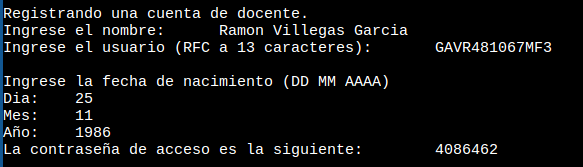
\includegraphics[width=.9\textwidth]{media/registro_docente.png}
    \caption{Opción de registrar docente.}
    \label{fig:regdoc}
\end{figure}

Ya que las funciones lógicas del programa están estrechamente relacionadas entres sí, la lógica del programa es: El sistema tendrá toda la información y los usuarios harán peticiones al sistema para realizar sus acciones.

A lo largo de todo el programa se trató de conservar el nombre de los métodos lo más descriptivo posible, utilizando la notación \textit{lowerCamel}, mientras que los atributos son de palabas completas separados por guión bajo, ésto con el fin de facilitar la lectura del código.

\begin{figure}[ht]
    \centering
    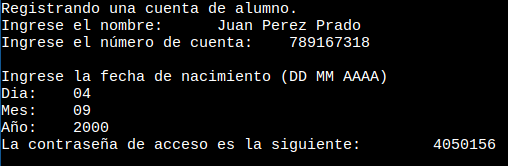
\includegraphics[width=.9\textwidth]{media/registrar_alumno.png}
    \caption{Opción de registrar alumno.}
    \label{fig:regalu}
\end{figure}

\subsection{Sistema.java}

“Sistema.java”, es el núcleo del sistema de inscripción. Esta clase contiene únicamente atributos estáticos siguiendo la lógica de que no se requiere instanciar objetos del tipo \textit{Sistema}, sino el sistema es único para todo usuario (así como la información almacenada). Es en el sistema donde se tiene la mayor parte de colecciones. En el análisis de datos abstractos sale a vista que existen tres clases independientes entre sí, docentes, alumnos y asignaturas\footnote{Si bien se podría considerar que alumnos y docentes pertenezcan a asignaturas, ésto no se puede decir de manera exclusiva, pues un alumno puede pertenecer a más de una asignatura y lo mismo con el profesor, un docente puede impartir más de una asignatura. Del mismo modo, decir que asignatura pertenece a profesor es incorrecto, pues una asignatura podría entonces pertenecer a más de un profesor y la composición de clases no se haría de manera correcta y recaería en volverse circular.}, mientras que la clase grupos pertenece exlcusivamente a la clase asignaturas. Una vez definida esta jerarquía se puede abordar las colecciones de datos, se decidió implementar conjuntos a través de \textit{HashSet} para almacenar tanto a alumnos como docentes de una forma que sea fácil de iterar, dichas colecciones se llaman \textit{alumnos\_totales} y \textit{docentes\_totales} respectivamente. Todos los alumnos son ubicados el sistema mediante su número de cuenta que será su usuario y los docentes mediante su RFC, por lo que la colección que almacena el objeto alumno con su usuario (número de cuenta) y la colección que almacena el objeto docente con su usario (RFC) requieren de búsqueda clave-valor y por tanto se implementan con la interfaz de mapas \textit{HashTable} llamdas \textit{clave\_alumnos} y \textit{clave\_docentes} respectivamente. Solo el sistema necesita de realizar búsqueda en estas colecciones, sin embargo la búsqueda de asignaturas ofrece búsqueda individual solicitada por el usuario, por lo que, además de relacionar objeto asignatura con clave asignatura, es necesario buscar el objeto asignatura por el nombre asignatura, ésto se triangulo con una colección que relaciona nombre asignatura con clave asignatura, entonces las colecciones correspondientes a asignaturas son: \textit{asignaturas\_totales}, \textit{clave\_asignaturas} y \textit{asignaturas}, siguiendo la convención de nombres anterior.\\

\begin{figure}[ht]
    \centering
    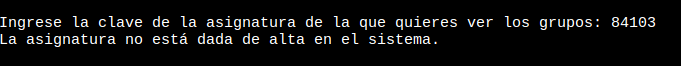
\includegraphics[width=.9\textwidth]{media/grupos_por_clave_mal.png}
    \caption{Error al ingresar clave de asignatura inexistente.}
    \label{fig:err1}
\end{figure}

Los métodos, todos estáticos, de la clase sistema juega con los modificadores de acceso privados si se trata de funcionalidades internas necesarias para otro métodos de la clase sistema, o pública si ofrece servicios de peticiones desde otras interfaces.

\begin{figure}[ht]
    \centering
    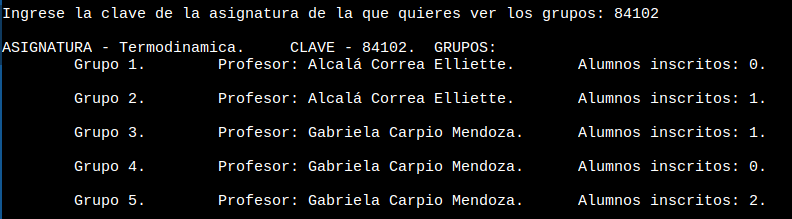
\includegraphics[width=.9\textwidth]{media/grupos_por_clave.png}
    \caption{Opción de imprimir grupos por clave.}
    \label{fig:gruposxclave}
\end{figure}

Entonces, la organización de los métodos de la clase sistema se puede agrupar en cuatro paquetes, en el código fuente cada uno se escuentra dividido por un comentario. El primero está reservado al menú principal, el segundo a la gestión de inicio de sesión y alta de usuarios como alumno, el tercero a la gestión de inicio de sesión y alta de usuarios como alumno (aunque algunos métodos se comparten entre ambos, alumno y docente), el cuarto al inicio de sesión como administrador, el quinto son \textit{request} o peticiones al sistema del resto de interfaces y el quinto a todo el manejo de abrir grupos y crear asignaturas, dar de alta y baja alumnos de grupos.\\

\begin{figure}[ht]
    \centering
    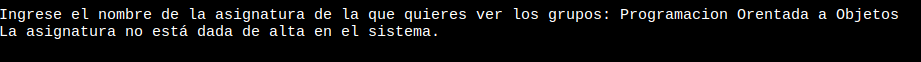
\includegraphics[width=.9\textwidth]{media/grupos_por_nombre_mal.png}
    \caption{Error al ingresar nombre de asignatura inexistente.}
    \label{fig:err2}
\end{figure}

Lo métodos del sistema cuentan con muy pocas validaciones de datos en algunas ocasiones y se limitan a realizar su función, dicha validación suele hacerse en las clases desde donde se mandan a llamar

\subsubsection{Menú principal}

El método \textbf{\textit{inicioSesion()}} es el punto de entrada principal al sistema. Permite a los usuarios iniciar sesión como alumno, docente o administrador, y luego los redirige a las opciones correspondientes.

\subsubsection{Ingreso alumnos}

Para los alumnos, el método \textbf{\textit{iniciarAlumno()}} maneja las opciones de inicio de sesión mediante \textbf{\textit{ingresarAlumno()}} para ingresar a una cuenta existente validando la contraseña, registrar una nueva cuenta a partir de \textbf{\textit{crearAlumno()}} para abrir un nuevo usuario (número de cuenta) que no esté registrado ya y asignar una contraseña, o de recuperar contraseña mediante \textbf{\textit{olvidoDeContraseña()}} para obtener la contraseña de un alumno registrado. También permite regresar al menú principal.

\begin{figure}[ht]
    \centering
    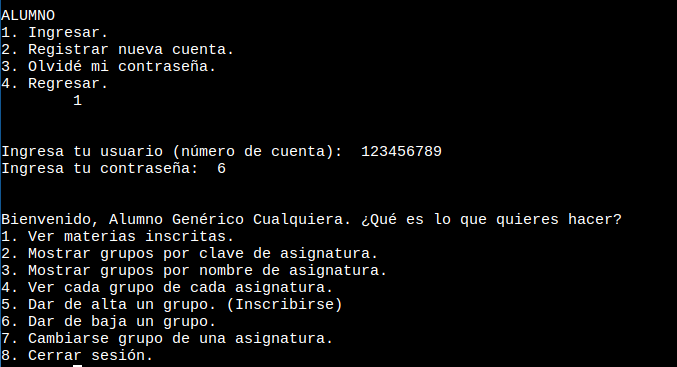
\includegraphics[width=.9\textwidth]{media/ingreso_alumno.png}
    \caption{Opción de ingresar como alumno.}
    \label{fig:ingresoalu}
\end{figure}

Si se crea un nuevo usuario se llamará al método de este mismo grupo \textbf{\textit{generarContraseña()}} que sirve de la misma forma para alumnos como docentes.

El método \textbf{\textit{olvidoDeContraseña()}} para recuperar la contraseña sigue la misma lógica y se invoca para alumnos y docentes.

\subsubsection{Ingreso docentes}

Para los docentes, el proceso es similar a como lo es en alumnos. El método \textbf{\textit{iniciarDocente()}} maneja las opciones de inicio de sesión, registro y olvido de contraseña. \textbf{\textit{ingresarDocente()}} permite a los docentes ingresar al sistema con su RFC y contraseña, mientras que \textbf{\textit{crearDocente()}} permite registrar una nueva cuenta de docente, leyendo su RFC y asignando una contraseña.

\begin{figure}[ht]
    \centering
    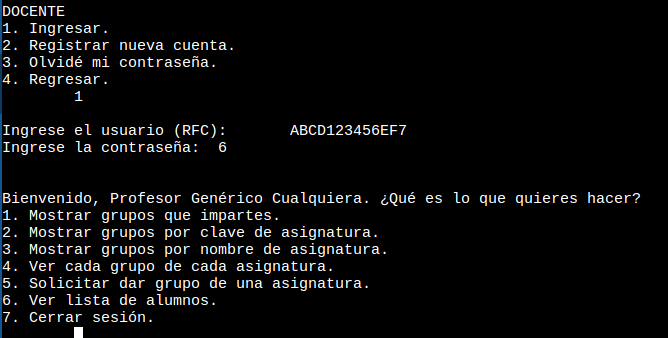
\includegraphics[width=.9\textwidth]{media/ingreso_docente.png}
    \caption{Opción de ingresar como docente.}
    \label{fig:ingresodoc}
\end{figure}

Como se mencionó, comparte los métodos \textbf{\textit{generarContraseña()}} y \textbf{\textit{olvidoDeContraseña()}} para el ingreso a alumnos.

De manera adicional, manda a llamar el método \textbf{\textit{isValid()}} cada vez que se lee el RFC para comprobar que la entrada sea, efectivamente, de trece caracteres.

\subsubsection{Ingreso administración}

El método \textbf{\textit{iniciarAdmin()}} permite al administrador iniciar sesión utilizando una contraseña predefinida y luego acceder a las funciones de administración del sistema. Su función es preguntar la contraseña, leerla y compararla con la predeterminada.

\begin{figure}[ht]
    \centering
    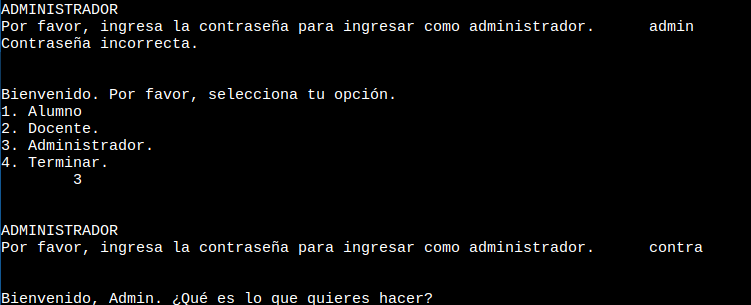
\includegraphics[width=.9\textwidth]{media/ingreso_admin.png}
    \caption{Opción de ingresar como administrador.}
    \label{fig:ingresoadm}
\end{figure}

\subsubsection{\textit{Requests} al sistema}

El método \textbf{\textit{imprimirAlumnos()}} recorre todo el conjunto de los alumnos totales imprimiendo para cada uno su nombre y número de cuenta o indica si no hay alumnos inscritos de ser el caso. \textbf{\textit{imprimirDocentes()}} hace lo mismo indicanto nombre y usuario (RFC) además de las materias que imparte cada grupo indicando su número de grupo; en caso de que no haya docentes dados de alta también lo indicará.

El método \textbf{\textit{imprimirAsignaturas()}} imprime cada grupo de cada asignatura, indicando el nombre de la asignatura, su clave única y cada uno de los grupos que tiene abiertos indicando el número de grupo, el profesor a cargo y el número de alumnos inscritos.

El método sobrecargado \textbf{\textit{imprimirGrupos()}} puede recibir como argumento la clave o nombre de una asignatura en específico y mostrará en pantalla todos los grupos de dicha asignatura de manera similar a como lo hace \textbf{\textit{imprimirAsignaturas()}}, mostrando nombre, clave y para cada grupo su número, docente a cargo y número de alumnos inscritos. Este método también es mandado a llamar por los métodos subsiguientes, \textbf{\textit{mostrarGruposPorClave()}} y \textbf{\textit{mostrarGruposPorNombre()}} cuya función es validar que la entrada pertenezca a un elemento en las colecciones correspondientes.

\subsubsection{Manejo de grupos y asignaturas}

El método \textbf{\textit{crearAsignatura()}} pide al usuario el nombre de la nueva asignatura asumiendo que no ingresará una existente y la agrega a las colecciones pertinentes asignándole una clave única en automático. Por otra parte, \textbf{\textit{abrirGrupo()}} se refiere a crear y añadir a las colecciones una nueva instancia de grupo, asignando un profesor designado, la clave de grupo será su número de grupo asignado en automático por el número de grupos que hay ya en la asignatura.

\begin{figure}[ht]
    \centering
    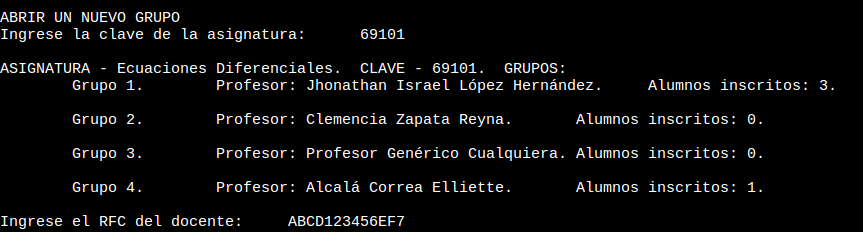
\includegraphics[width=.9\textwidth]{media/abrir_grupo.png}
    \caption{Opción de abrir nuevo grupo.}
    \label{fig:abrir_grupo}
\end{figure}

Finalmente, los métodos \textbf{\textit{altaGrupo()}} y \textbf{\textit{bajaGrupo()}} dan de alta o baja a un alumno (inscribir o desinscribir), respectivamente, añadiendo o eliminando al alumno de las colecciones correspondientes y actualizando los atributos de número de alumnos inscritos en un grupo según se deba. Cuentan con la opción de mostrar en pantalla o no cuando un alumno se ha inscrito de manera satisfactoria. El último método de la clase \textbf{\textit{cambiarGrupo()}} invoca los dos métodos anteriores de manera consecutiva para inscribir al alumno en el grupo de su elección.

\subsection{Admin.java}

Dentro de la clase “Admin.java” un administrador puede realizar diversas acciones como registrar alumnos, docentes, asignaturas, y abrir grupos por medio de los métodos descritos anteriormente de la clase sistema. La clase contiene un método estático \textbf{\textit{iniciar()}} que sirve como punto de entrada, presentando un menú de opciones al usuario y ejecutando las acciones correspondientes a la selección. Se emplea la clase \textbf{\textit{Scanner}} para capturar la entrada del usuario desde la consola o el teclado.

\begin{figure}[ht]
    \centering
    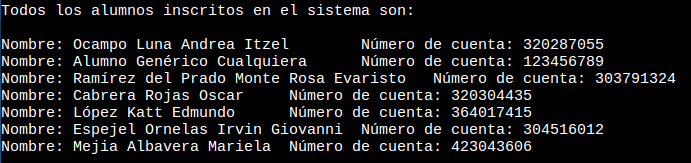
\includegraphics[width=.9\textwidth]{media/alumnos.png}
    \caption{Opción de mostrar todos los alumnos dados de alta en el sistema.}
    \label{fig:mostrara_alumnos}
\end{figure}

El menú de opciones ofrece al administrador diez acciones diferentes, desde registrar alumnos hasta cerrar sesión. Para el conjunto de opciones se utiliza una estructura de control \textit{switch-case} que dirige el flujo del programa hacia el método adecuado.

\begin{figure}[ht]
    \centering
    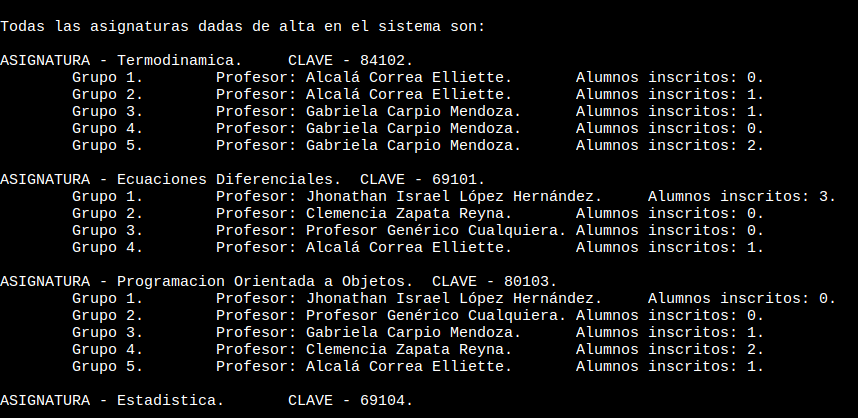
\includegraphics[width=.9\textwidth]{media/asignaturas.png}
    \caption{Opción de mostrar todas las asignaturas dadas de alta en el sistema.}
    \label{fig:abrir_grupo}
\end{figure}

El caso \textbf{\textit{nuevoGrupo()}} permite al administrador abrir un nuevo grupo, solicitando la clave de la asignatura y el RFC del docente. Una vez proporcionados estos datos y si pertenecen a objetos dados de alta en el sistema, el método llama a la función \textbf{\textit{abrirGrupo()}} de la clase Sistema para crear el grupo correspondiente.

\begin{figure}[ht]
    \centering
    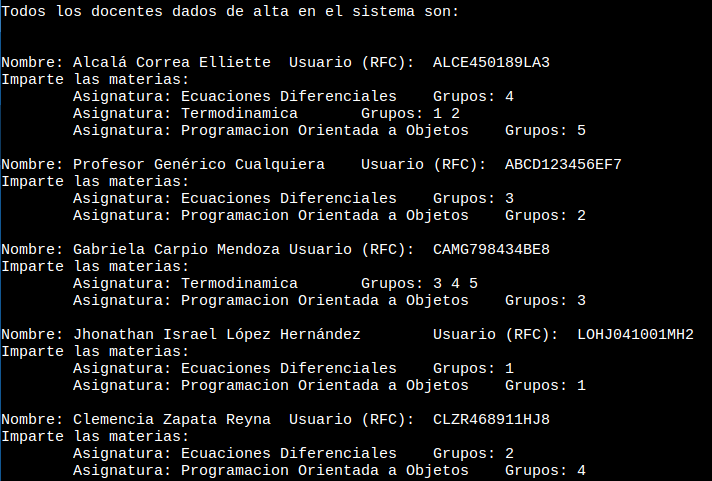
\includegraphics[width=.9\textwidth]{media/docentes.png}
    \caption{Opción de mostrar todos los docentes en el sistema.}
    \label{fig:mostrar_docentes}
\end{figure}

El programa incluye un mecanismo para manejar situaciones donde el usuario introduce una opción no válida. En tal caso, se imprime un mensaje de error y se vuelve al método \textbf{\textit{iniciar()}} para volver a mostrar el menú de opciones y poder reintentarlo en dado caso.

\subsection{Alumnos.java}

La clase llamada \textit{Alumnos.java}, representa a todos los estudiantes de la Facultad de Ingeniería (F.I.). Cada instancia de esta clase almacena información como el número de cuenta, nombre, contraseña y los grupos en los que está inscrito el alumno.

\begin{figure}[ht]
    \centering
    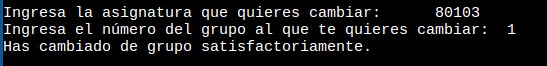
\includegraphics[width=.9\textwidth]{media/cambiar_asignatura.png}
    \caption{Opción de cambiarse de grupo una asignatura.}
    \label{fig:cambiar_asig}
\end{figure}

El método \textbf{\textit{opciones()}} es el punto de entrada principal para los alumnos, mostrando un menú de opciones que permite al estudiante realizar diversas acciones como ver las materias inscritas, mostrar grupos por clave o nombre de asignatura, dar de alta o baja un grupo, cambiar de grupo o cerrar sesión. Este método utiliza un objeto \textbf{\textit{Scanner}} para capturar la entrada del usuario desde la consola o el teclado.

\begin{figure}[ht]
    \centering
    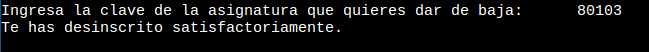
\includegraphics[width=.9\textwidth]{media/desinscribir_asignatura.png}
    \caption{Opción de desinscribir un grupo.}
    \label{fig:desinscribir_asig}
\end{figure}

Para el conjunto de opciones del menú se emplea una estructura \textit{switch-case} para dirigir el flujo del programa hacia el método correspondiente. Por ejemplo, el caso \textbf{\textit{imprimirMateriasInscritas()}} muestra las materias en las que está inscrito el alumno, mientras que los casos \textbf{\textit{inscribir()}}, \textbf{\textit{desinscribir()}} y \textbf{i} permiten al alumno interactuar con los grupos de asignaturas.

\begin{figure}[ht]
    \centering
    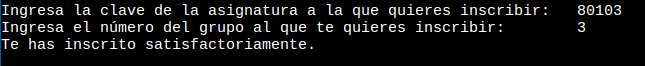
\includegraphics[width=.9\textwidth]{media/inscribir_asignatura.png}
    \caption{Opción de inscribir una asignatura.}
    \label{fig:inscribir}
\end{figure}

El método \textbf{\textit{inscribir()}} solicita al alumno la clave de la asignatura y el número de grupo al que desea inscribirse, verificando la existencia de los datos de entrada e invocando el método del sistema \textbf{\textit{altaGrupo()}} si todo está bien. De manera similar, \textbf{\textit{desinscribir()}} y \textbf{\textit{cambiarGrupo()}} permiten al alumno darse de baja de un grupo o cambiar de grupo respectivamente, con validaciones para asegurar que la acción sea válida, de ser así se invoca entonces a los métodos del sistema \textbf{\textit{bajaGrupo()}} y \textbf{\textit{cambiarGrupo()}}.

\begin{figure}[ht]
    \centering
    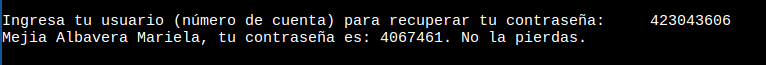
\includegraphics[width=.9\textwidth]{media/olvido_de_contrasena.png}
    \caption{Opción de olvido de contraseña.}
    \label{fig:olvido}
\end{figure}

Esta clase contiene métodos de acceso \textit{getters} y \textit{setters} para seguir el concepto del encapsulamiento.

\begin{figure}[ht]
    \centering
    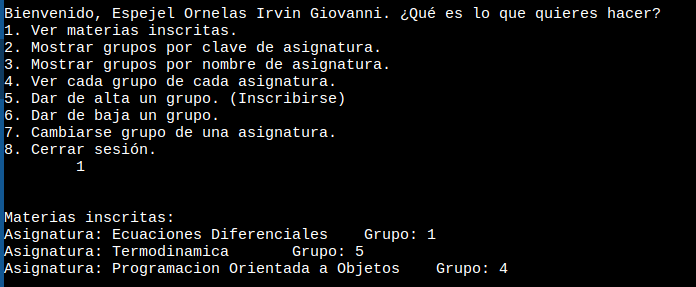
\includegraphics[width=.9\textwidth]{media/ver_materias_inscritas.png}
    \caption{Opción de ver materias inscritas.}
    \label{fig:matins}
\end{figure}

\subsection{Profesores.java}

La clase \textit{Profesores.java}, representa a todos los profesores que imparten clase en la F.I.

\begin{figure}[ht]
    \centering
    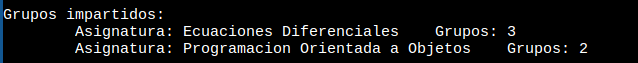
\includegraphics[width=.9\textwidth]{media/grupos_impartidos.png}
    \caption{Opción de mostrar grupos que imparte un profesor.}
    \label{fig:grupos_impartidos}
\end{figure}

Cada instancia de esta clase almacena información como el nombre del profesor, su usuario (RFC), la clave de acceso al sistema, y una lista de listas que indica cada grupo de cada asignatura que el profesor imparte.

El constructor de la clase permite inicializar un profesor con su usuario, nombre y clave de acceso al sistema.

La clase cuenta con métodos de acceso \textit{getters} y \textit{setters} para acceder y modificar los atributos del profesor, como el nombre, la clave y la lista de grupos que imparte.

\begin{figure}[ht]
    \centering
    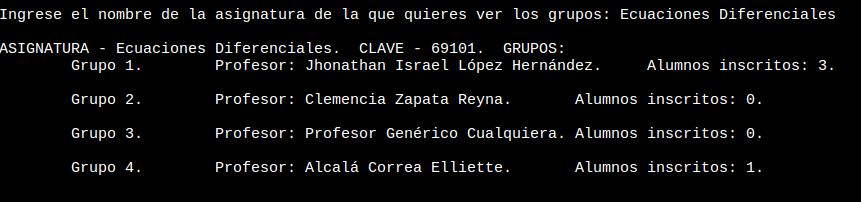
\includegraphics[width=.9\textwidth]{media/grupos_por_nombre.png}
    \caption{Opción de imprimir grupos de una asignatura por su nombre.}
    \label{fig:gruposxnombre}
\end{figure}

El método \textit{opciones()} es el punto de entrada principal para los profesores, mostrando un menú de opciones que permite al profesor realizar diversas acciones, como mostrar los grupos que imparte, mostrar grupos por clave o nombre de asignatura, solicitar dar grupo de una asignatura, ver la lista de alumnos o cerrar sesión.

Para cada opción del menú, se emplea una estructura \textit{switch-case} para dirigir el flujo del programa hacia el método correspondiente. Por ejemplo, el caso \textbf{\textit{mostrarGruposImpartidos()}} muestra los grupos que el profesor imparte, mientras que \textbf{\textit{solicitarImpartir()}} permite al profesor solicitar impartir un nuevo grupo una cierta asignatura.

Esta clase contiene métodos de acceso \textit{getters} y \textit{setters} para seguir el concepto del encapsulamiento.

\subsection{Grupos.java}

La clase \textit{Grupos.java}, representa el grupo de estudiantes inscritos en una asignatura. 

Cada instancia de esta clase almacena información como el número de alumnos inscritos, el número de grupo, y el nombre del profesor a cargo.

La clase cuenta con métodos de acceso \textit{getters} y \textit{setters} para acceder y modificar los atributos de los grupos, como el número de grupo, el número de alumnos inscritos, la lista de alumnos inscritos y el nombre del profesor.

La lista de alumnos inscritos se implementa utilizando una \textit{LinkedList}, lo que permite almacenar eficientemente un número variable de alumnos en cada grupo.

\subsection{Materias.java}

La clase \textit{Materias.java}, representa las asignaturas impartidas en la F.I. Cada instancia de esta clase almacena información como la clave de la asignatura, el nombre y una lista de grupos asociados a esa asignatura.

La clase cuenta con constructores que permiten inicializar una asignatura con su nombre y opcionalmente con su clave y lista de grupos. También incluye métodos de acceso \textit{getters} y \textit{setters} para acceder y modificar los atributos de la asignatura, como el nombre, la clave y la lista de grupos.

El método \textbf{\textit{generarClave()}} se encarga de generar una clave única para la asignatura utilizando el primer carácter del nombre y el número total de asignaturas dadas de alta en el sistema. El funcionamiento haca que no existan claves repetidas.

\subsection{Sistema\_de\_inscripcion.java}

La clase Sistema\_de\_inscripcion.java, es un punto de entrada principal para todo el programa al estar dentro del método estático \textit{main()} que se encarga de llamar al método estático \textit{inicioSesion()} de la clase Sistema.

La única función que cumple esta clase, además de dar inicio al funcionamiento del programa, es la de iniciarlizar con ciertos elementos las colecciones, sean éstos alumnos, docentes, asignaturas, grupos e inscripción de alumnos en grupos. De requerir lo contrario se pueden comentar las líneas de código 5-88 de esta clase para probar el funcionamiento del programa sin datos iniciales.

El método \textit{main()} es el punto de entrada principal de cualquier programa Java.

\section{Conclusiones}

\subsection{Cabrera Rojas Oscar}

Los objetivos se cumplieron satisfactoriamente, el alumno conoció los principales aspectos de las colecciones en Java, lo que son, la jerarquía que siguen, los métodos y atributos de cada una, su propósito general y a utilizar cada una según sea conveniente por las necesidades del programa; aplicó los conocimientos adquiridos en la implementación de un programa que simula el sistema de inscripción de la Facultad de Ingeniería utilizando los conceptos básicos de la programación orientada a objetos.

El programa resultó ser mucho más complejo de los realizados en la asignatura hasta la fecha, requirió comprender conceptos de la programación orientada a objetos tales como: abstracción, encapsulamiento, modularidad, cohesión, \textit{casteo} de datos, métodos de acceso, referncias \textit{this} a la clase, métodos constructores, métodos y variables de clase, utlierías y clases de uso general y composición de clases. Ver una aplicación conjunta práctica de dichos conceptos donde el funcionamiento depende constantemente entre ellas definitivamente contribuyó al aprendizaje del alumno respecto a los temas mencionados. De la misma forma ocurre con las colecciones en Java, la investigación pasó de lo meramente teórico a lo práctico, asegurando para el alumno su pleno entendimiento y dominio.

\subsection{Espejel Ornelas Irvin Giovanni}

Las colecciones en Java son componentes esenciales en el desarrollo de software, ya que nos permiten manejar eficientemente grupos de elementos relacionados. Desde listas hasta conjuntos y mapas, estas estructuras nos brindan la flexibilidad y funcionalidad necesarias para abordar una amplia gama de problemas de programación. 

Es crucial comprender las diferencias entre las diferentes implementaciones de colecciones, así como sus ventajas y limitaciones. Cada tipo de colección tiene su propósito y ofrece características específicas que pueden afectar el rendimiento y la eficiencia de nuestros programas. 

Además, la elección de la implementación de colección adecuada depende en gran medida de los requisitos del problema que estamos tratando de resolver. Ya sea que necesitemos mantener un orden específico, evitar duplicados o asociar claves con valores, es importante seleccionar la estructura de datos más apropiada para nuestras necesidades.

\subsection{López Katt Edmundo}

Las colecciones en Java son sin duda un pilar fundamental en el desarrollo de software, brindando a los programadores una gama versátil de herramientas para manipular datos de manera eficiente y efectiva. Desde listas hasta conjuntos y mapas, estas estructuras de datos ofrecen una amplia variedad de funcionalidades que pueden adaptarse a una diversidad de problemas y escenarios de programación.

Una de las principales diferencias entre las diferentes implementaciones de colecciones radica en su estructura interna y en las operaciones que admiten de manera eficiente. Por ejemplo, las listas, como ArrayList y LinkedList, son adecuadas para situaciones donde se necesita un acceso rápido a elementos individuales o donde se requieren operaciones de inserción y eliminación frecuentes en cualquier punto de la lista. Por otro lado, los conjuntos, como HashSet y TreeSet, son ideales para eliminar duplicados y verificar la pertenencia de elementos rápidamente, mientras que los mapas, como HashMap y TreeMap, son útiles para asociar claves con valores y realizar búsquedas rápidas por clave.

Al elegir la implementación de colección adecuada, es crucial considerar varios factores, como el rendimiento, la complejidad temporal de las operaciones y los requisitos específicos del problema. Por ejemplo, si se necesita mantener un orden específico en los elementos o si la aplicación requiere operaciones de búsqueda frecuentes, puede ser más adecuado utilizar un TreeMap en lugar de un HashMap. Del mismo modo, si se necesitan eliminar duplicados o garantizar la unicidad de elementos, un HashSet puede ser la elección más apropiada.

Además, es importante tener en cuenta el uso adecuado de tipos genéricos en Java para garantizar la seguridad y la coherencia de los datos almacenados en las colecciones. Utilizar tipos genéricos nos permite especificar el tipo de elementos que contendrá la colección, lo que ayuda a prevenir errores de tipo en tiempo de compilación y mejora la legibilidad y mantenibilidad del código.

\bibliographystyle{acm}
\bibliography{main, api}

\end{document}

